% move all configuration stuff into includes file so we can focus on the content
\documentclass[aspectratio=169,hyperref={pdfpagelabels=false,colorlinks=true,linkcolor=white,urlcolor=blue},t]{beamer}

%%%%%%%%%%%%%%%%%%%%%%%%%%%%%%%%%%%%%%%%%%%%%%%%%%%%%%%%%%%%%%%%%%%%%%%%%%%%%%%%%%
%%%%%%%%%%%%%%%%%%%%%%%%%%%%%%%%%%%%%%%%%%%%%%%%%%%%%%%%%%%%%%%%%%%%%%%%%%%%%%%%%%
% packages
\usepackage{pict2e}
\usepackage{epic}
\usepackage{amsmath,amsfonts,amssymb}
\usepackage{units}
\usepackage{fancybox}
\usepackage[absolute,overlay]{textpos} 
\usepackage{media9} % avi2flv: "C:\Program Files\ffmpeg\bin\ffmpeg.exe" -i TuneFreqFilterbank.avi -b 600k -s 441x324 -r 15 -acodec copy TuneFreqFilterbank.flv
\usepackage{animate}
\usepackage{gensymb}
\usepackage{multirow}
\usepackage{silence}
\usepackage[backend=bibtex,style=ieee]{biblatex}
\AtEveryCitekey{\iffootnote{\tiny}{}}
\addbibresource{references}

%%%%%%%%%%%%%%%%%%%%%%%%%%%%%%%%%%%%%%%%%%%%%%%%%%%%%%%%%%%%%%%%%%%%%%%%%%%%%%%%%%
%%%%%%%%%%%%%%%%%%%%%%%%%%%%%%%%%%%%%%%%%%%%%%%%%%%%%%%%%%%%%%%%%%%%%%%%%%%%%%%%%%
% relative paths
\graphicspath{{graph/}}


%%%%%%%%%%%%%%%%%%%%%%%%%%%%%%%%%%%%%%%%%%%%%%%%%%%%%%%%%%%%%%%%%%%%%%%%%%%%%%%%%%
%%%%%%%%%%%%%%%%%%%%%%%%%%%%%%%%%%%%%%%%%%%%%%%%%%%%%%%%%%%%%%%%%%%%%%%%%%%%%%%%%%
% units
\setlength{\unitlength}{1mm}

%%%%%%%%%%%%%%%%%%%%%%%%%%%%%%%%%%%%%%%%%%%%%%%%%%%%%%%%%%%%%%%%%%%%%%%%%%%%%%%%%%
%%%%%%%%%%%%%%%%%%%%%%%%%%%%%%%%%%%%%%%%%%%%%%%%%%%%%%%%%%%%%%%%%%%%%%%%%%%%%%%%%%
% theme & layout
\usetheme{Frankfurt}
\beamertemplatenavigationsymbolsempty
%\setbeamertemplate{frametitle}[smoothbars theme]
\setbeamertemplate{frametitle}
{
    \begin{beamercolorbox}[ht=1.8em,wd=\paperwidth]{frametitle}
        \vspace{-.1em}%
        \hspace{.2em}{\strut\insertframetitle\strut}
        
        \hspace{.2em}\small\strut\insertframesubtitle\strut
        %\hfill
        %
\includegraphics[height=.8cm,keepaspectratio]{CenterMusicTechnology-solid-2lines-white-CoAtag}
        
    \end{beamercolorbox}
    \begin{textblock*}{100mm}(11.6cm,.7cm)
        \includegraphics[height=.8cm,keepaspectratio]{logo_GTCMT_black}
    \end{textblock*}
}

% set this to ensure bulletpoints without subsections
\usepackage{remreset}
\makeatletter
\@removefromreset{subsection}{section}
\makeatother
\setcounter{subsection}{1}

%---------------------------------------------------------------------------------
% appearance
\setbeamercolor{structure}{fg=gtgold}
\setbeamercovered{transparent} %invisible
\setbeamercolor{bibliography entry author}{fg=black}
\setbeamercolor*{bibliography entry title}{fg=black}
\setbeamercolor*{bibliography entry note}{fg=black}

%\usepackage{pgfpages}
%\setbeameroption{show notes}
%\setbeameroption{show notes on second screen=right}
%---------------------------------------------------------------------------------
% fontsize
\let\Tiny=\tiny

%%%%%%%%%%%%%%%%%%%%%%%%%%%%%%%%%%%%%%%%%%%%%%%%%%%%%%%%%%%%%%%%%%%%%%%%%%%%%%%%%%
%%%%%%%%%%%%%%%%%%%%%%%%%%%%%%%%%%%%%%%%%%%%%%%%%%%%%%%%%%%%%%%%%%%%%%%%%%%%%%%%%%
% warnings
\pdfsuppresswarningpagegroup=1
\WarningFilter{biblatex}{Patching footnotes failed}
\WarningFilter{latexfont}{Font shape}
\WarningFilter{latexfont}{Some font shapes}
\WarningFilter{gensymb}{Not defining}


%%%%%%%%%%%%%%%%%%%%%%%%%%%%%%%%%%%%%%%%%%%%%%%%%%%%%%%%%%%%%%%%%%%%%%%%%%%%%%%%%%
%%%%%%%%%%%%%%%%%%%%%%%%%%%%%%%%%%%%%%%%%%%%%%%%%%%%%%%%%%%%%%%%%%%%%%%%%%%%%%%%%%
% title information
\title[]{Introduction to Audio Content Analysis}   
\author[alexander lerch]{alexander lerch} 
%\institute{~}
%\date[Alexander Lerch]{}
\titlegraphic{\vspace{-16mm}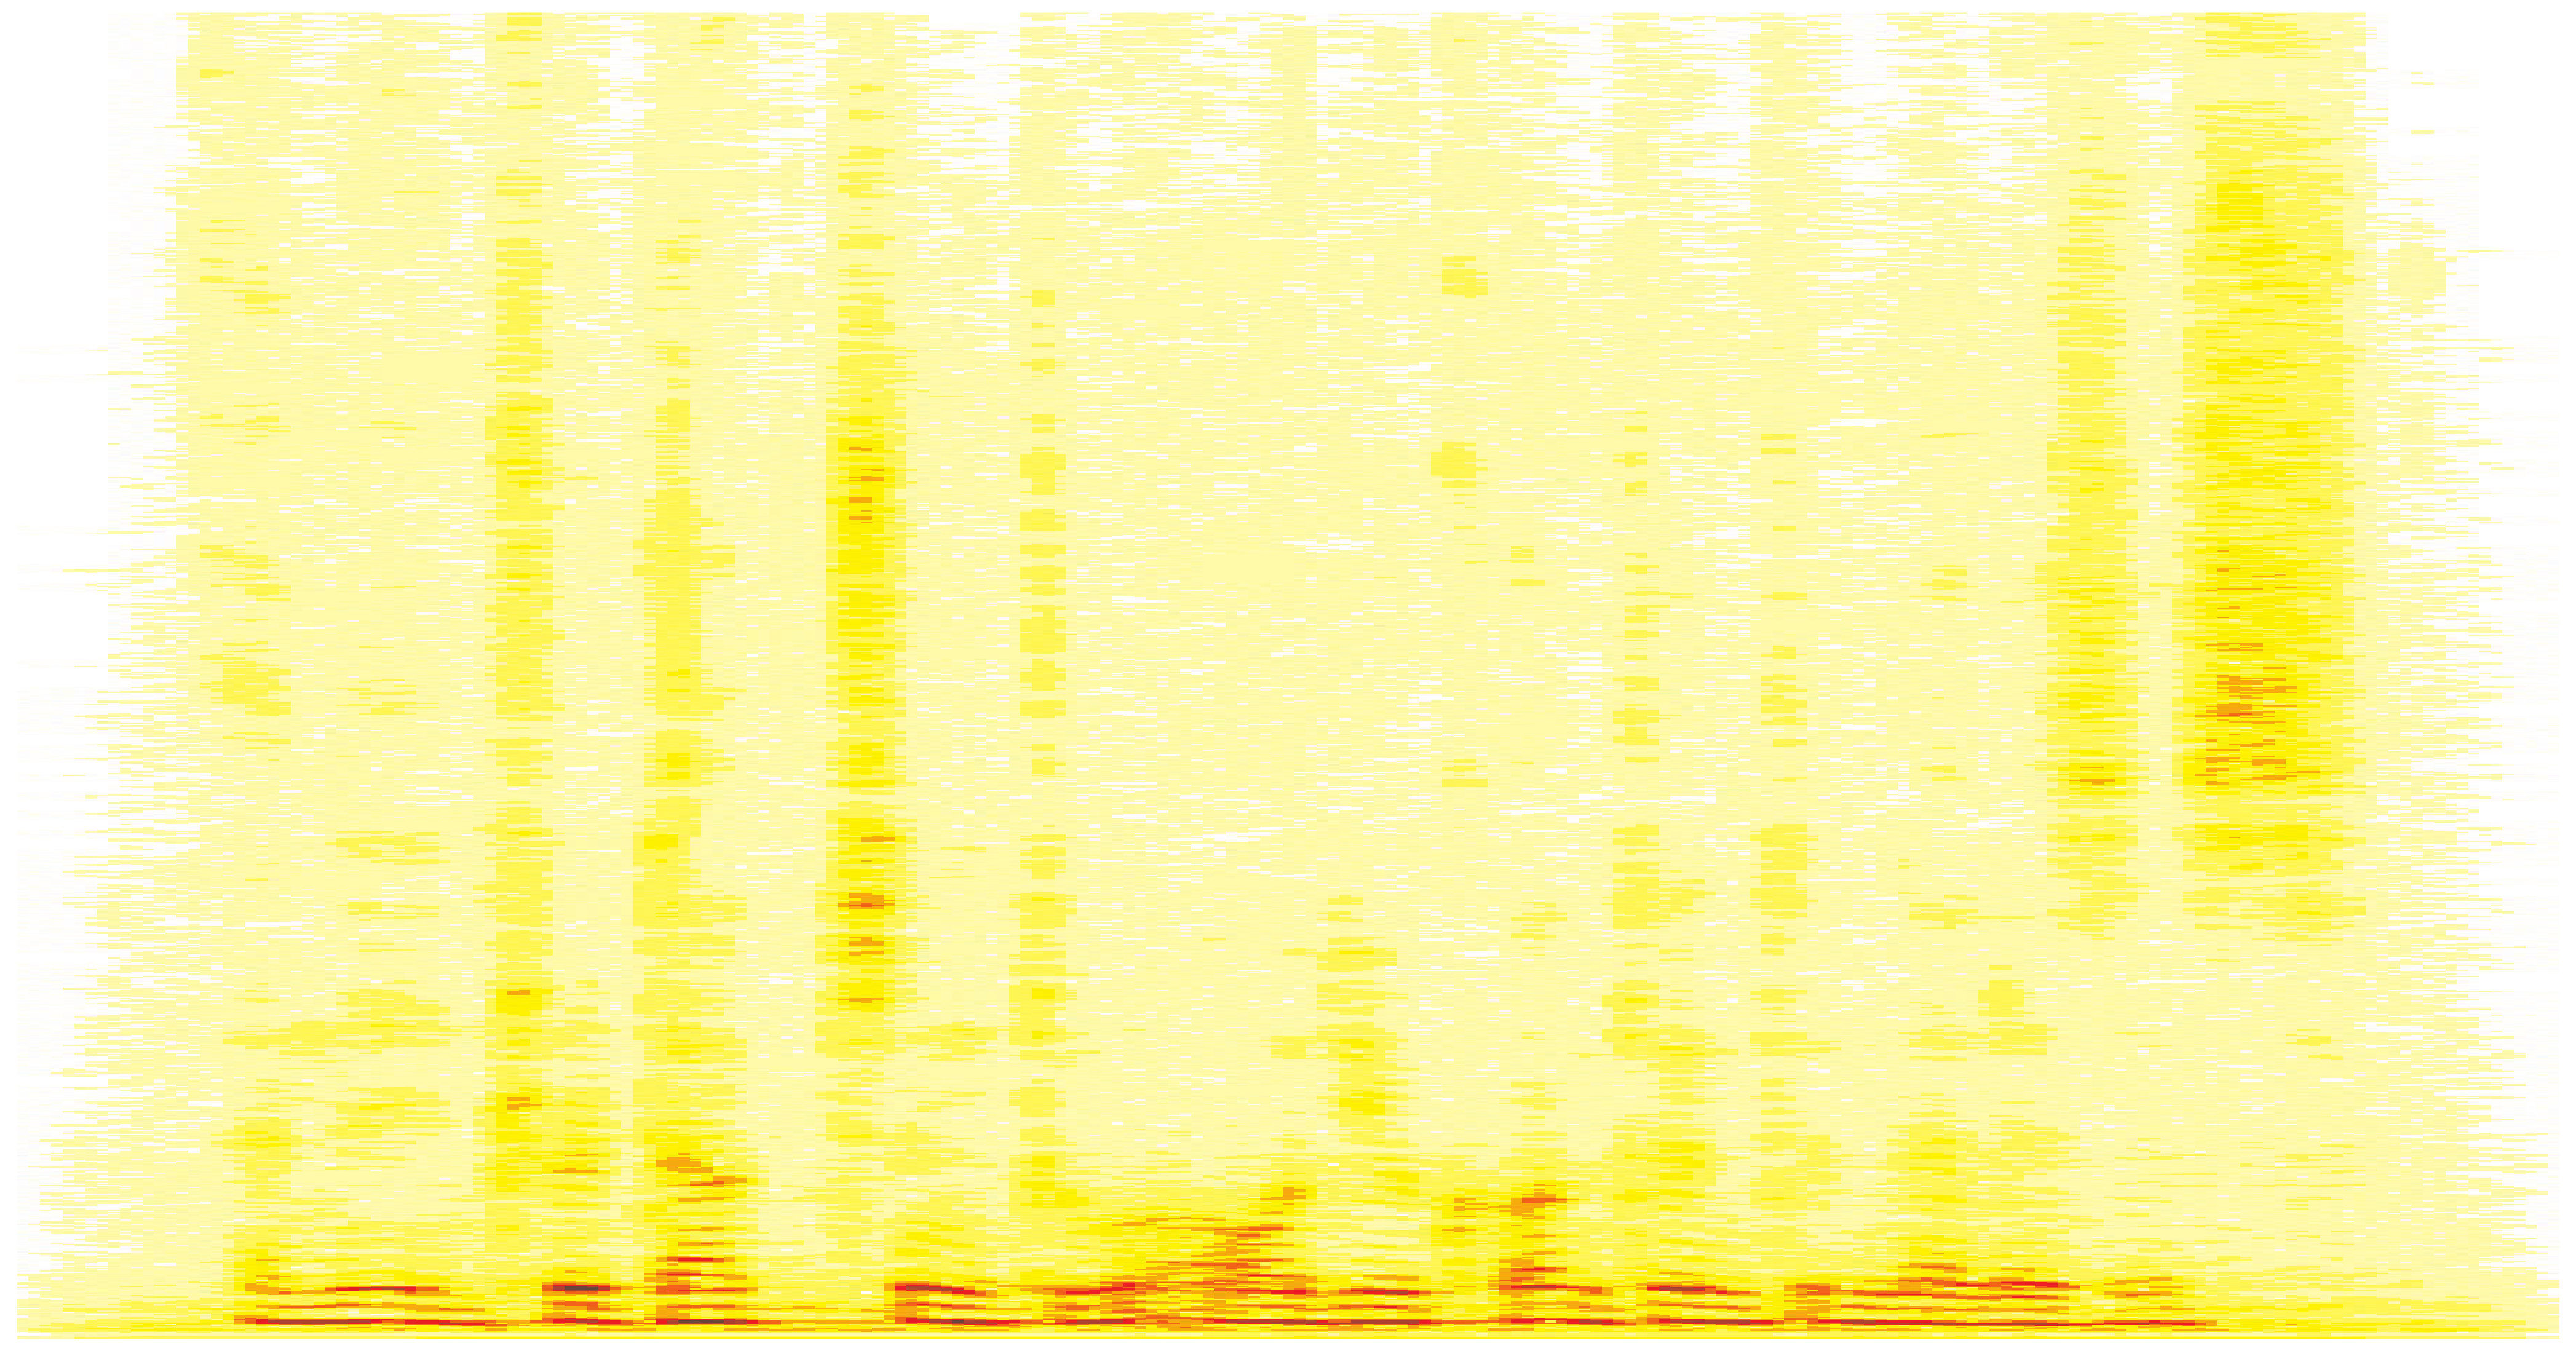
\includegraphics[width=\textwidth,height=3cm]{title}}

%%%%%%%%%%%%%%%%%%%%%%%%%%%%%%%%%%%%%%%%%%%%%%%%%%%%%%%%%%%%%%%%%%%%%%%%%%%%%%%%%%
%%%%%%%%%%%%%%%%%%%%%%%%%%%%%%%%%%%%%%%%%%%%%%%%%%%%%%%%%%%%%%%%%%%%%%%%%%%%%%%%%%
% colors
\definecolor{gtgold}{HTML}{E0AA0F} %{rgb}{0.88,0.66,1,0.06} [234, 170, 0]/256

%%%%%%%%%%%%%%%%%%%%%%%%%%%%%%%%%%%%%%%%%%%%%%%%%%%%%%%%%%%%%%%%%%%%%%%%%%%%%%%%%%
%%%%%%%%%%%%%%%%%%%%%%%%%%%%%%%%%%%%%%%%%%%%%%%%%%%%%%%%%%%%%%%%%%%%%%%%%%%%%%%%%%
% math
\DeclareMathOperator*{\argmax}{argmax}
\DeclareMathOperator*{\argmin}{argmin}
\DeclareMathOperator*{\atan}{atan}
\DeclareMathOperator*{\arcsinh}{arcsinh}
\DeclareMathOperator*{\sign}{sign}
\DeclareMathOperator*{\tcdf}{tcdf}
\DeclareMathOperator*{\si}{sinc}
\DeclareMathOperator*{\princarg}{princarg}
\DeclareMathOperator*{\arccosh}{arccosh}
\DeclareMathOperator*{\hwr}{HWR}
\DeclareMathOperator*{\flip}{flip}
\DeclareMathOperator*{\sinc}{sinc}
\DeclareMathOperator*{\floor}{floor}
\newcommand{\e}{{e}}
\newcommand{\jom}{\mathrm{j}\omega}
\newcommand{\jOm}{\mathrm{j}\Omega}
\newcommand   {\mat}[1]    		{\boldsymbol{\uppercase{#1}}}		%bold
\renewcommand {\vec}[1]    		{\boldsymbol{\lowercase{#1}}}		%bold

%%%%%%%%%%%%%%%%%%%%%%%%%%%%%%%%%%%%%%%%%%%%%%%%%%%%%%%%%%%%%%%%%%%%%%%%%%%%%%%%%%
%%%%%%%%%%%%%%%%%%%%%%%%%%%%%%%%%%%%%%%%%%%%%%%%%%%%%%%%%%%%%%%%%%%%%%%%%%%%%%%%%%
% media9
\newcommand{\includeaudio}[1]{{\includemedia[
                        addresource=audio/#1.mp3,
                        width=5mm,
                        height=5mm,
                        activate=onclick,
                        flashvars={
                            source=audio/#1.mp3  
                            &autoPlay=true
                        }]
                        {
\includegraphics[width=5mm, height=5mm]{SpeakerIcon}}
                        {APlayer.swf}}}
\newcommand{\audioautoplay}[1]{{\begin{center}\includemedia[
                            addresource=audio/#1.mp3,
                            width=.1\linewidth,
                            height=.01\linewidth,
                            activate=pageopen,
                            flashvars={
                                source=audio/#1.mp3  
                                &autoPlay=true
                            }]
                            {}
                            {APlayer.swf}\end{center}}}

\newcommand{\includevideo}[1]{{\begin{center}\includemedia[
                        addresource=video/#1.mp4,
                        width=0.8\linewidth,
                        height=0.4\linewidth,
                        activate=onclick,
                        flashvars={
                            source=video/#1.mp4  
                            &autoPlay=true
                        }]
                        {}
                        {VPlayer.swf}\end{center}}}
\newcommand{\videowithmatlab}[1]{{\begin{center}\includemedia[
                        addresource=video/animate#1.mp4,
                        width=0.8\linewidth,
                        height=0.4\linewidth,
                        activate=onclick,
                        flashvars={
                            source=video/animate#1.mp4  
                            &autoPlay=true
                        }]
                        {}
                        {VPlayer.swf}\end{center}\addreference{matlab source: matlab/animate#1.m}}}
                        

%%%%%%%%%%%%%%%%%%%%%%%%%%%%%%%%%%%%%%%%%%%%%%%%%%%%%%%%%%%%%%%%%%%%%%%%%%%%%%%%%%
%%%%%%%%%%%%%%%%%%%%%%%%%%%%%%%%%%%%%%%%%%%%%%%%%%%%%%%%%%%%%%%%%%%%%%%%%%%%%%%%%%
% other commands
\newcommand{\question}[1]{%\vspace{-4mm}
                          \setbeamercovered{invisible}
                          \begin{columns}[T]
                            \column{.8\textwidth}
                                \textbf{#1}
                            \column{.2\textwidth}
                                \vspace{-8mm}
                                \begin{flushright}
                                     
\includegraphics[scale=.5]{question_mark}
                                \end{flushright}
                                \vspace{6mm}
                          \end{columns}\pause\vspace{-12mm}}

\newcommand{\toremember}[1]{%\vspace{-4mm}
                          \begin{columns}[T]
                            \column{.8\textwidth}
                                \textbf{#1}
                            \column{.2\textwidth}
                                \vspace{-4mm}
                                \begin{flushright}
                                     
\includegraphics[scale=.5]{exclamation_mark}
                                \end{flushright}
                                \vspace{6mm}
                          \end{columns}\vspace{-6mm}}

\newcommand{\matlabexercise}[1]{%\vspace{-4mm}
                          \setbeamercovered{invisible}
                          \begin{columns}[T]
                            \column{.8\textwidth}
                                \textbf{matlab exercise}: #1
                            \column{.2\textwidth}
                                \begin{flushright}
                                     
\includegraphics[scale=.5]{logo_matlab}
                                \end{flushright}
                                %\vspace{6mm}
                          \end{columns}}

\newcommand{\addreference}[1]{  
                  
                    \begin{textblock*}{\baselineskip }(1.12\textwidth,.3\textheight) %(1.15\textwidth,.4\textheight)
                        \rotatebox{90}{\tiny {#1}}
                    \end{textblock*}}
                    
\newcommand{\figwithmatlab}[1]{
                    \begin{figure}
                        \centering
                        \includegraphics{#1}
                        %\label{fig:#1}
                    \end{figure}
                    
                    \addreference{matlab source: \href{https://github.com/alexanderlerch/ACA-Slides/blob/master/matlab/display#1.m}{matlab/display#1.m}}}
\newcommand{\figwithref}[2]{
                    \begin{figure}
                        \centering
                        \includegraphics{#1}
                        \label{fig:#1}
                    \end{figure}
                    
                    \addreference{#2}}  
                                    
\newcommand{\inserticon}[1]{

                    \begin{textblock*}{100mm}(14.5cm,7.5cm)
                        \includegraphics[height=.8cm,keepaspectratio]{#1}
                    \end{textblock*}}            

%%%%%%%%%%%%%%%%%%%%%%%%%%%%%%%%%%%%%%%%%%%%%%%%%%%%%%%%%%%%%%%%%%%%%%%%%%%%%%%%%%
%%%%%%%%%%%%%%%%%%%%%%%%%%%%%%%%%%%%%%%%%%%%%%%%%%%%%%%%%%%%%%%%%%%%%%%%%%%%%%%%%%
% counters
\newcounter{i}
\newcounter{j}
\newcounter{iXOffset}
\newcounter{iYOffset}
\newcounter{iXBlockSize}
\newcounter{iYBlockSize}
\newcounter{iYBlockSizeDiv2}
\newcounter{iDistance}



\subtitle{Module 5.1: Terminology \& Notation of Pitch}

%%%%%%%%%%%%%%%%%%%%%%%%%%%%%%%%%%%%%%%%%%%%%%%%%%%%%%%%%%%%%%%%%%%%%%%%%%%%
\begin{document}
    % generate title page
	

\begin{frame}
    \titlepage
    %\vspace{-5mm}
    \begin{flushright}
        \href{http://www.gtcmt.gatech.edu}{\includegraphics[height=.8cm,keepaspectratio]{logo_GTCMT_black}}
    \end{flushright}
\end{frame}


    \section[overview]{lecture overview}
        \begin{frame}{introduction}{overview}
            \begin{block}{corresponding textbook section}
                    \href{http://ieeexplore.ieee.org/xpl/articleDetails.jsp?arnumber=6331122}{Chapter 5~---~Tonal Analysis}: pp.~82--91
            \end{block}

            \begin{itemize}
                \item   \textbf{lecture content}
                    \begin{itemize}
                        \item   pitch-related music terminology: interval, mode, tonic, chord
                    \end{itemize}
                \bigskip
                \item<2->   \textbf{learning objectives}
                    \begin{itemize}
                        \item   name musical intervals and notate them in score notation
                        \item   explain pitch distance
                        \item   discuss whether a chord is a harmony
                    \end{itemize}
            \end{itemize}
            \inserticon{directions}
        \end{frame}

    \section[musical pitch]{pitch in music}
        \begin{frame}{musical pitch}{notation and names}
            
            each octave (freq factor $2$) is split into $12$ pitch classes
            \begin{columns}
            \column{0.35\linewidth}
            \begin{figure}
            \scalebox{.8}
            {
                \begin{footnotesize}
\begin{picture}(70,40)
	\setcounter{iXOffset}{0}
	\setcounter{iYOffset}{5}
	\setcounter{iXBlockSize}{10}
	\setcounter{iYBlockSize}{35}

	% white keys
	\put(\value{iXOffset}, \value{iYOffset})
		{\framebox(\value{iXBlockSize}, \value{iYBlockSize})[b] {\footnotesize{\shortstack[c]{$C$\\ \ }}}}

	\addtocounter{iXOffset}{\value{iXBlockSize}}
	\put(\value{iXOffset}, \value{iYOffset})
		{\framebox(\value{iXBlockSize}, \value{iYBlockSize})[b] {\footnotesize{\shortstack[c]{$D$\\ \ }}}}

	\addtocounter{iXOffset}{\value{iXBlockSize}}
	\put(\value{iXOffset}, \value{iYOffset})
		{\framebox(\value{iXBlockSize}, \value{iYBlockSize})[b] {\footnotesize{\shortstack[c]{$E$\\ \ }}}}

	\addtocounter{iXOffset}{\value{iXBlockSize}}
	\put(\value{iXOffset}, \value{iYOffset})
		{\framebox(\value{iXBlockSize}, \value{iYBlockSize})[b] {\footnotesize{\shortstack[c]{$F$\\ \ }}}}

	\addtocounter{iXOffset}{\value{iXBlockSize}}
	\put(\value{iXOffset}, \value{iYOffset})
		{\framebox(\value{iXBlockSize}, \value{iYBlockSize})[b] {\footnotesize{\shortstack[c]{$G$\\ \ }}}}

	\addtocounter{iXOffset}{\value{iXBlockSize}}
	\put(\value{iXOffset}, \value{iYOffset})
		{\framebox(\value{iXBlockSize}, \value{iYBlockSize})[b] {\footnotesize{\shortstack[c]{$A$\\ \ }}}}
	\addtocounter{iXOffset}{\value{iXBlockSize}}
	
	\put(\value{iXOffset}, \value{iYOffset})
		{\framebox(\value{iXBlockSize}, \value{iYBlockSize})[b] {\footnotesize{\shortstack[c]{$B$\\ \ }}}}

	\setcounter{iDistance}{\value{iXBlockSize}}
	\setcounter{iXOffset}{7}
	\setcounter{iYOffset}{16}
	\setcounter{iXBlockSize}{3}
	\setcounter{iYBlockSize}{23}
	
	\put(\value{iXOffset}, \value{iYOffset})
		{\colorbox{black}{ \framebox(\value{iXBlockSize}, \value{iYBlockSize})[b] {\footnotesize{\shortstack[c]{\textcolor {white}{$C\sharp$}\\ \textcolor {white}{$D\flat$}\\ \ }}}}}

	\addtocounter{iXOffset}{\value{iDistance}}
	
	\put(\value{iXOffset}, \value{iYOffset})
		{\colorbox{black}{ \framebox(\value{iXBlockSize}, \value{iYBlockSize})[b] {\footnotesize{\shortstack[c]{\textcolor {white}{$D\sharp$}\\ \textcolor {white}{$E\flat$}\\ \ }}}}}

	\addtocounter{iXOffset}{\value{iDistance}}
	\addtocounter{iXOffset}{\value{iDistance}}
	
	\put(\value{iXOffset}, \value{iYOffset})
		{\colorbox{black}{ \framebox(\value{iXBlockSize}, \value{iYBlockSize})[b] {\footnotesize{\shortstack[c]{\textcolor {white}{$F\sharp$}\\ \textcolor {white}{$G\flat$}\\ \ }}}}}

	\addtocounter{iXOffset}{\value{iDistance}}
	
	\put(\value{iXOffset}, \value{iYOffset})
		{\colorbox{black}{ \framebox(\value{iXBlockSize}, \value{iYBlockSize})[b] {\footnotesize{\shortstack[c]{\textcolor {white}{$G\sharp$}\\ \textcolor {white}{$A\flat$}\\ \ }}}}}

	\addtocounter{iXOffset}{\value{iDistance}}
	
	\put(\value{iXOffset}, \value{iYOffset})
		{\colorbox{black}{ \framebox(\value{iXBlockSize}, \value{iYBlockSize})[b] {\footnotesize{\shortstack[c]{\textcolor {white}{$A\sharp$}\\ \textcolor {white}{$B\flat$}\\ \ }}}}}

\end{picture}
\end{footnotesize}

            }
            \end{figure}
            \column{0.5\linewidth}
            \begin{figure}
                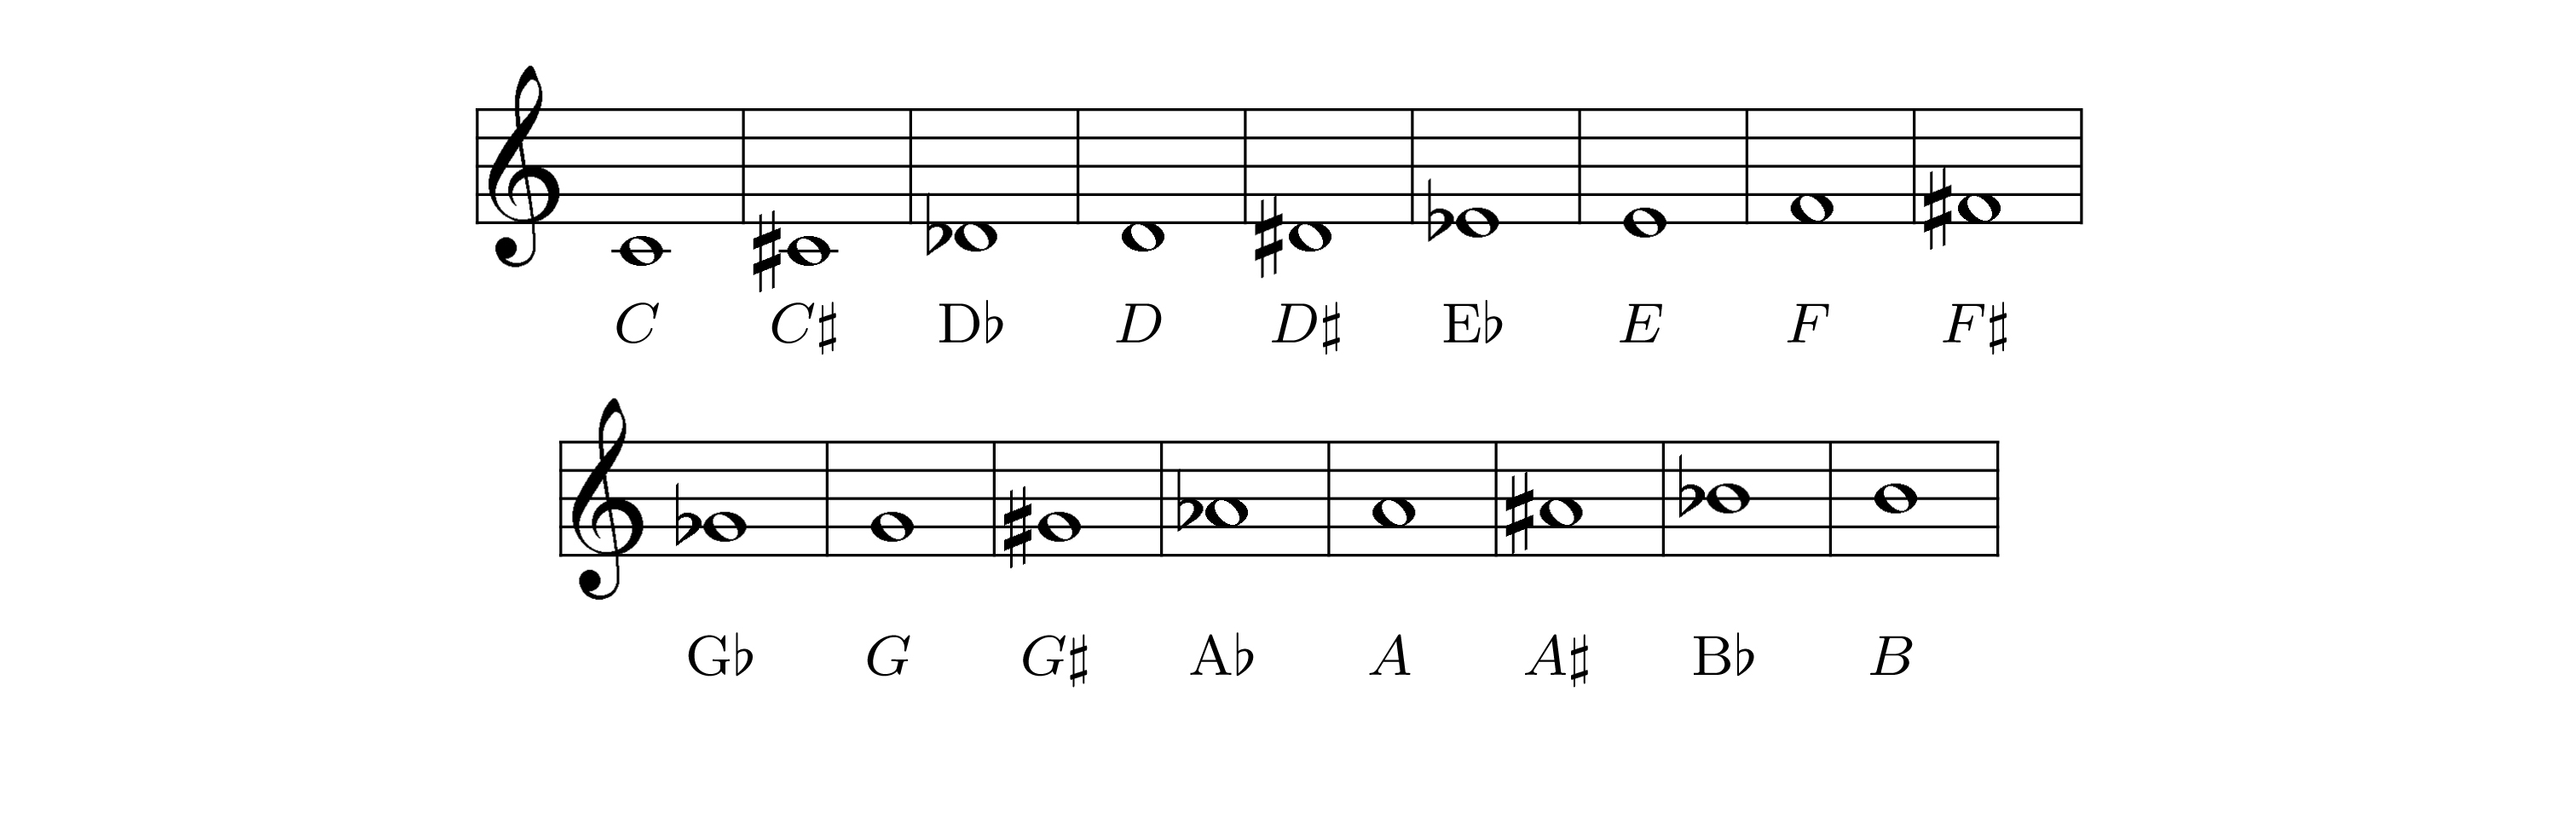
\includegraphics{pitch_pitches}
            \end{figure}
            \end{columns}

            \begin{footnotesize}
                \begin{table}
                    \centering
                    \begin{tabular}{cccccccccccc} %{\textwidth}{@{\extracolsep{\fill}}ccccccccccccc}
                        \\ \hline
                        \bf{\emph{$0$}}	 & \bf{\emph{$1$}}	 & \bf{\emph{$2$}}	 & \bf{\emph{$3$}}	 & \bf{\emph{$4$}}	 & \bf{\emph{$5$}}	 & \bf{\emph{$6$}}	 & \bf{\emph{$7$}}	 & \bf{\emph{$8$}}	 & \bf{\emph{$9$}}	 & \bf{\emph{$10$}}	 & \bf{\emph{$11$}}\\ 
                         \hline
                        \bf{$C$}	 & $C\sharp / D\flat$	 & $D$	 & $D\sharp / E\flat$	 & E	 & $F$	 & $F\sharp / G\flat$	 & $G$	 & $G\sharp / A\flat$	 & $A$	 & $A\sharp / B\flat$	 & $B$\\
                    \end{tabular}
                \end{table}
            \end{footnotesize}
        \end{frame}
        
        %\begin{frame}{musical pitch}{ --- pitch classes 2/2}
            %\begin{footnotesize}
                %\begin{table}
                    %\centering
                    %\begin{tabular}{cccccccccccc} %{\textwidth}{@{\extracolsep{\fill}}ccccccccccccc}
                        %\\ \hline
                        %\bf{\emph{Index}}	 & \bf{\emph{Name}}	 & \bf{\emph{Solf\'ege Name}}	 & \bf{\emph{$\Delta\mathrm{ST}$}}\\ 
                         %\hline
                        %\bf{$0$}	 & $C$	 & Do	 & 1\\
                        %\bf{$2$}	 & $D$	 & Re	 & 2\\
                        %\bf{$4$}	 & $E$	 & Mi	 & 2\\
                        %\bf{$5$}	 & $F$	 & Fa	 & 1\\
                        %\bf{$7$}	 & $G$	 & Sol	 & 2\\
                        %\bf{$9$}	 & $A$	 & La	 & 2\\
                        %\bf{$11$}	 & $B$	 & Si	 & 2\\
                    %\end{tabular}
                %\end{table}
            %\end{footnotesize}
        %\end{frame}

    \section{intervals}
        \begin{frame}{musical pitch}{intervals}
            \vspace{-8mm}
            \begin{columns}
            \column{0.47\linewidth}
            \begin{scriptsize}
                \begin{table}
                    \centering
                    \begin{tabular}{lccccccccccc} %{\textwidth}{@{\extracolsep{\fill}}ccccccccccccc}
                        \\ \hline
                        \bf{\emph{Interval}}	 & \bf{\emph{Enharmonic Equivalent}}	 & \bf{\emph{$\Delta\mathrm{ST}$}}\\ 
                         \hline
                        \bf{Unison}	 & Diminished Second	 & 0\\
                        \bf{Minor Second}	 & Augmented Unison	 & 1\\
                        \bf{(Major) Second}	 & Diminished Third	 & 2\\
                        \bf{Minor Third}	 & Augmented Second	 & 3\\
                        \bf{Major Third}	 & Diminished Fourth	 & 4\\
                        \bf{(Perfect) Fourth}	 & Augmented Third	 & 5\\
                        \bf{Augmented Fourth}	 & Diminished Fifth/Tritone	 & 6\\
                        \bf{(Perfect) Fifth}	 & Diminished Sixth	 & 7\\
                        \bf{Minor Sixth}	 & Augmented Fifth	 & 8\\
                        \bf{Major Sixth}	 & Diminished Seventh	 & 9\\
                        \bf{Minor Seventh}	 & Augmented Sixth	 & 10\\
                        \bf{Major Seventh}	 & Diminished Octave	 & 11\\
                        \bf{(Perfect) Octave}	 & Augmented Seventh	 & 12\\
                    \end{tabular}
                \end{table}
            \end{scriptsize}
            \column{0.5\linewidth}
            \begin{figure}
                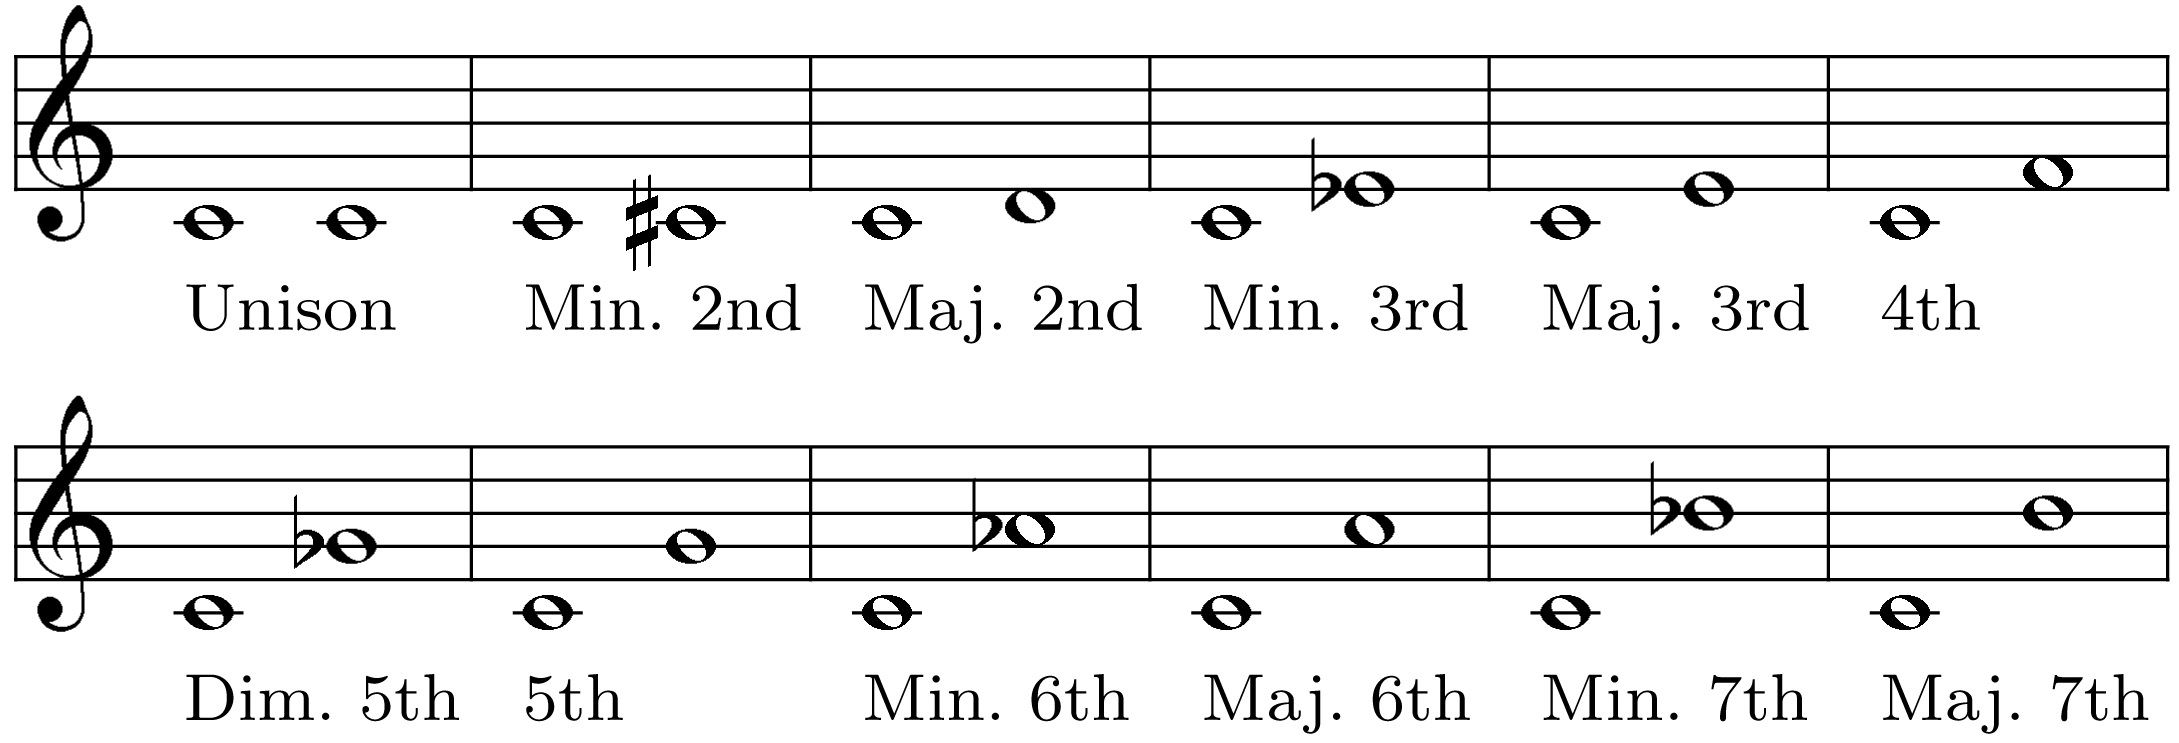
\includegraphics[scale=.8]{pitch_intervals}
            \end{figure}
            \end{columns}
        \end{frame}


    \section{MIDI pitch}
        \begin{frame}{musical pitch}{ MIDI pitch}
                \begin{eqnarray*}\label{eq:midi_pitch}
                    \mathfrak{p}(f) &=& 69 + 12\cdot\log_2\left(\frac{f}{f_\mathrm{A4}}\right) \\
                    f(\mathfrak{p}) &=& f_{A4}\cdot2^{\frac{\mathfrak{p}-69}{12}}
                \end{eqnarray*}
                
                \pause
                MIDI pitch mapping to \textit{pitch class}
                \begin{equation*}\label{eq:pcidx}
                    \mathrm{PC}(\mathfrak{p}) = \mod(\mathfrak{p}, 12) 
                \end{equation*}
                
        \end{frame}
    
    \section{Cent}
        \begin{frame}{musical pitch}{  (MIDI) pitch distance}
                \textbf{cent}: pitch distance between two frequencies
                \begin{footnotesize}
                \begin{eqnarray*}\label{eq:cent}
                    \Delta C(f_1,f_2)	&=& 100\cdot\big(\mathfrak{p}(f_1) - \mathfrak{p}(f_2)\big)\\
                                        \pause
                                        &=& 100\cdot\left(\left(69 + 12\cdot\log_2\left(\frac{f_1}{f_{A4}}\right)\right) - \left(69 + 12\cdot\log_2\left(\frac{f_2}{f_{A4}}\right)\right)\right)\\
                                        \pause
                                        &=& 1200\cdot\log_2\left( \frac{f_1}{f_2} \right) 
                \end{eqnarray*}
                \end{footnotesize}
                \bigskip
                $\Rightarrow$ $\unit[100]{cents}$ span one semitone
        \end{frame}
        
    \section{temperament}
        \begin{frame}{musical pitch}{ temperament}
            \begin{itemize}
                \item	equally tempered scale:
                    \begin{itemize}
                        \item   octave split into 12 equidistant notes (on log scale)
                        \item   not key dependent,any modulation possible
                        \item   enharmonic equivalence: $C\sharp = D\flat$
                        \item   typical scale for keyboard instruments
                    \end{itemize}
                    


                %\item<3->	deviations of other scales
                    %\begin{tiny}\begin{table}
                        %\centering
                        %\begin{tabular}{lcccccc} %{c|p{12mm}p{12mm}p{12mm}p{12mm}p{12mm}p{12mm}p{12mm}}
                            %\\ \hline
                            %\bf{\emph{Pitch Class}}	 & \bf{\emph{Equally}}	 & \bf{\emph{Pythagorean}}	 & \bf{\emph{Meantone}}	 & \bf{\emph{Diatonic Major}}	 & \bf{\emph{Diatonic Minor}}\\ 
                             %\hline
                            %\bf{$C$}	 & $0$	 & $0$	 & $0$	 & $0$	 & $0$\\
                            %\bf{$C^\#$}	 & $0$	 & $-$	 & $-$	 & $-$	 & $-$\\
                            %\bf{$D$}	 & $0$	 & $+3.9$	 & $-6.9$	 & $+3.9$	 & $+3.9$\\
                            %\bf{$E^b$}	 & $0$	 & $-$	 & $-$	 & $-$	 & $+15.6$\\
                            %\bf{$E$}	 & $0$	 & $+7.8$	 & $-13.7$	 & $-13.7$	 & $-$\\
                            %\bf{$F$}	 & $0$	 & $-2.0$	 & $+3.4$	 & $-2.0$	 & $-2.0$\\
                            %\bf{$F^\#$}	 & $0$	 & $-$	 & $-$	 & $-$	 & $-$\\
                            %\bf{$G$}	 & $0$	 & $+2.0$	 & $-3.5$	 & $+2.0$	 & $+2.0$\\
                            %\bf{$A^b$}	 & $0$	 & $-$	 & $-$	 & $-$	 & $+13.7$\\
                            %\bf{$A$}	 & $0$	 & $+5.9$	 & $-10.2$	 & $-15.6$	 & $-$\\
                            %\bf{$B^b$}	 & $0$	 & $-$	 & $-$ 	 & $-$	 & $+17.6$\\
                            %\bf{$B$}	 & $0$	 & $+9.8$	 & $-17.1$	 & $-11.7$	 & $-$\\
                        %\end{tabular}
                    %\end{table}\end{tiny}			
            \end{itemize}
            \bigskip
            
            \begin{equation*}
                \frac{f_1}{f_2} = 2^{\nicefrac{N}{12}} 
            \end{equation*}
            
             \begin{itemize}
                \item	other scales can sound purer for specific keys but are less commonly used
            \end{itemize}
       \end{frame}
        
    \section{intonation}
        \begin{frame}{musical pitch}{ intonation \& vibrato}
            \begin{itemize}
                \item	\textbf{expressive intonation}: deviation of pitch frequency from temperament depending on musical context
                        \begin{itemize}
                            \item	leading tones
                            \item	``pure'' intervals
                        \end{itemize}

                \item<2->	\textbf{vibrato}
                        \begin{itemize}
                            \item	periodic modulation around mean pitch
                            \pause
                            \item 	frequency: app. 4--10 \unit{Hz}, range: app. 20--300 \unit{cents}	
                        \end{itemize}
                \bigskip
                \item<3-> applies only to instruments with
                    \begin{itemize}
                        \item<4->   continuous frequency scales: vocals, string instruments, trombone, \ldots
                        \item<5->   other possibilities to adjust frequency: guitar, wind instruments, \ldots
                    \end{itemize}
            \end{itemize}
        \end{frame}
        
    \section{summary}
        \begin{frame}{summary}{lecture content}
            \begin{itemize}
                \item   \textbf{pitch}
                    \begin{itemize}
                        \item   each octave split into 12 pitches
                        \item   \textit{pitch class} is an octave-independent representation of pitch
                    \end{itemize}
                \smallskip
                \item   \textbf{intervals}
                    \begin{itemize}
                        \item   distance between two pitches
                    \end{itemize}
                \smallskip
                \item   \textbf{cent}
                    \begin{itemize}
                        \item   metric for pitch distance
                    \end{itemize}
            \end{itemize}
            \inserticon{summary}
        \end{frame}
\end{document}
